\chapter{Beam Background Model} \label{ch:beam_bg}

The MuSun beam line includes an electrostatic beam kicker known as the muon on request system.
This device diverts the beam after a muon entrance is observed, reducing the muon entrance rate by a large factor during the 25 $\mu s$ kick window.  
The kicker is instrumental in reaching our target statistics by allowing an increased beam rate while minimizing pileup events.
However, in doing so it introduces a time dependence into the beam-related backgrounds which is correlated with the muon entrance times.

\section{Kicker Time Dependence}

Muons can only trigger the kicker and be counted as good entrances if they do not enter during the kicker window of a previous entrance.
Therefore, the beam must be in the un-kicked state at the muon entrance time.  
The muon then fires the kicker, and another good entrance cannot occur until the kicker deactivates 25 $\mu s$ later.

Immediately after the kicker window ends, muons will begin entering the detector at the full un-kicked beam rate.  
The first muon to be observed after this will be the next good entrance and trigger the next kicker firing.
Determining the time distribution of the next kick is then a simple exercise in poisson statistics.
If the muon beam rate is $\lambda_b$, then the probability of n events occurring in a time t is given by the formula
\begin{equation}
P(n,t) = \frac{(\lambda_b t)^n}{n!} e^{-\lambda_b t}.
\end{equation}
Now, for the next muon that triggers the kicker, we want zero events to occur before time t and then one event to occur within a short interval dt
\begin{align}
P(t) dt & = P(0,t) * P(1,dt) = e^{-\lambda_b t} * (\lambda_b dt) e^{-\lambda_b t} \\
P(t) & = \lambda_b e^{-\lambda_b t}.
\end{align}

So far, I have been considering the delay before the next muon entrance, but the individual muon entrances are identical.
Therefore, the same time distribution also describes the separation between a given entrance and the previous entrance.
By integrating the probability above, we find the probability of observing the un-kicked beam at any given time relative to the entrance:
\begin{equation}
P_b(t) = \begin{cases} e^{\lambda_b t}        & -t_k+t_{\mu}<t<0 \\
                       1                      & 0<t<t_{\mu} \\
                       0                      & t_{\mu}<t<t_k-t_{\mu} \\
                       1                      & t_k-t_{\mu}<t<t_k \\
                       e^{-\lambda_b (t-t_k)} & t_k<t<2 t_k-t_{\mu} \end{cases}
\label{eq:kicker}
\end{equation}
where I have introduced the kicker window time $t_k \approx 25 \mu s$, and the kicker response delay time of $t_{\mu} \approx 800 ns$ for muons.

Finally, some minor adjustments to this formulation are required due to the presence of the muon clock.
Because the muon clock can fire the kicker, the effective beam rate is the sum of the true muon entrance rate and the clock rate.
The clock my also produce very complicated background behavior if the rate is set too high, due to the clock "entrances" always occurring with a fixed separation.
Although above I have stopped at modeling the kicks before and after the primary stop, correlations persist for several additional entrances before washing out.
If the clock rate is high enough that a clock event occurs before the effects of the previous even have decayed, this can set up a periodic oscillation in the beam.
The entrance autocorrelations appear to die away by 200 $\mu s$ though, so clock rates of 5 kHz or lower should be unaffected.

\begin{figure}[h]
  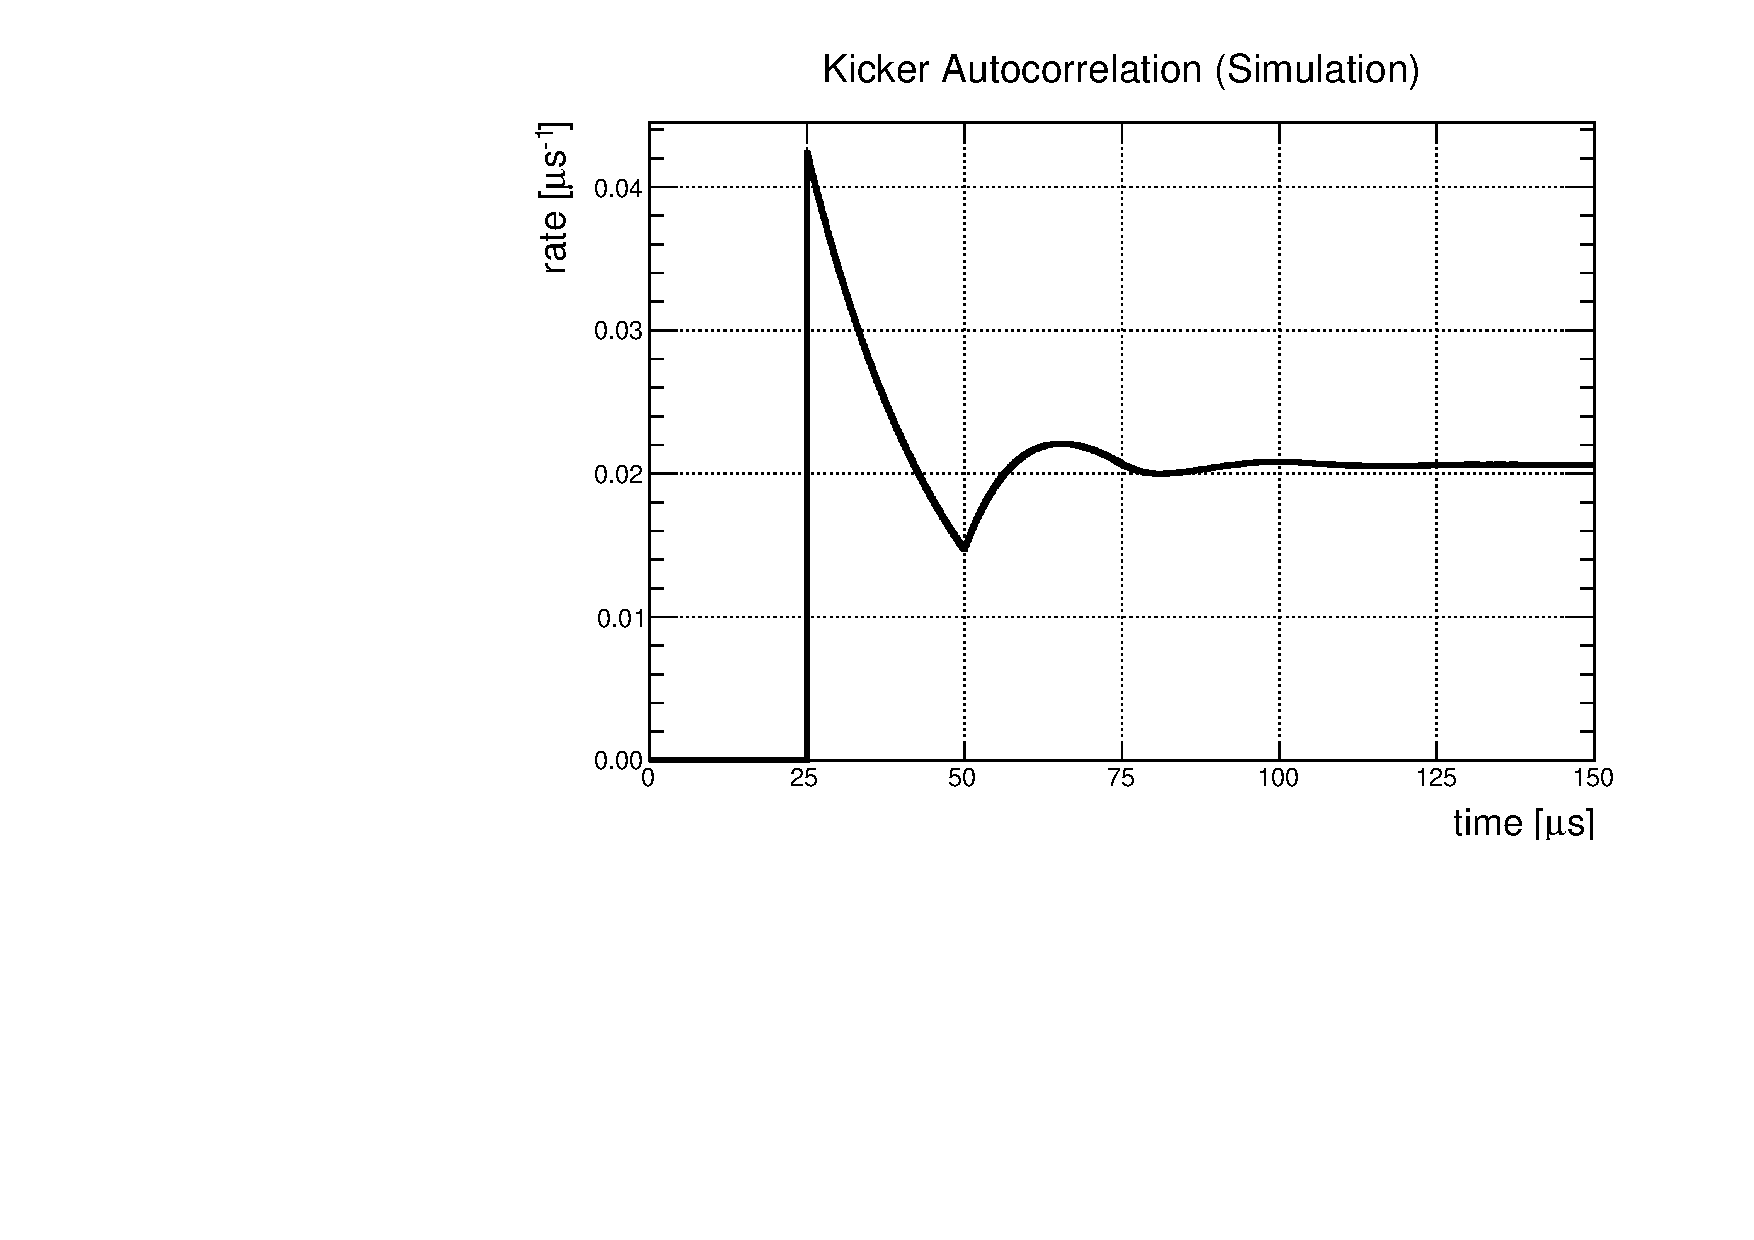
\includegraphics[width=\textwidth]{beam/figures/KickAutoCorrSim.pdf}
  \caption{Entrance autocorrelation simulation}
  \label{fig:entrance_long}
\end{figure}

\section{Muon Background}

A given background may be characterized by two entrance rates, one for the normal beam and one for when the beam is kicked.
Furthermore, the accelerator produces a characteristic RF oscillation in the beam, the amplitude of which may vary between the kicked and un-kicked configurations.
The oscillation phase varies between background signals, and may also be affected by the kick although this has not been observed.
%todo - check whether electron oscillations change phase.

The time dependance of most backgrounds follows directly from the kicker time distribution.
However, the muons are special because muon entrances trigger the kicker.
In particular, we distinguish muons which are "seen" or "unseen" by the MuPC detector.  
To be clear, "unseen" muons may still be detected by the MuSC or other detectors, the classification is determined solely by the MuPC.  

Unseen muons include muons missed due to detector inefficiency, but also muons that are somewhat off-axis and miss the MuPC entirely.
These muons clearly cannot trigger the kicker, so they follow the kicker time distribution.
Seen muons that enter after the current entrance time also cannot fire the kicker since the kicker has already been fired by the current entrance.  
However, it is impossible for a seen muon to occur between the end of the previous kick window and the start of the next event, since it would then fire the kicker and become the next event itself.
This can be modeled by setting the un-kicked background rate to zero for seen muons before the entrance time.

The instantaneous step function in equation \ref{eq:kicker} is clearly unphysical, and should be replaced with a continuous function.  
The transition between the kicked and un-kicked states could potentially be rather complicated, and depends on the rate that the kicker charges up and the beam profile.  
A non-uniform or misaligned beam could even produce a transient spike in the rate as the kicker briefly sweeps the beam across the detector.
Substantial effort has gone into tuning the beam though, so I simply use an error function with a parameter $\sigma$ to control the width:

\begin{equation}
P_{b,\mu}(t) = \begin{cases} e^{\lambda_b t}        & -t_k+t_{\mu}<t<0 \\
                       1 - \frac{1}{2} erf(\frac{t-t_{\mu}}{\sigma}) + \frac{1}{2} erf(\frac{t-(t_k-t_{\mu})}{\sigma}) & 0<t<t_k \\
                       e^{-\lambda_b (t-t_k)}   & t_k<t<2 t_k-t_{\mu} \end{cases}
\label{eq:kicker_muon}
\end{equation}

The kicker response time $t_{\mu}$ mentioned above is the sum of two different delays.  
A signal is immediately sent to activate the kicker after an entrance is observed, but there is a delay as the signal travels along the wire.
After the kicker diverts the beam, there is an additional delay as particles that have already passed the kicker continue to travel down the beam pipe to the detector.
Together, these effects produce a total delay of 800 $ns$ before the muon entrance rate is reduced by the kick.

Finally, the seen and unseen muon background rates are given by the equations:
\begin{align}
R_{\mu,s}(t) & = [A + B sin(\omega_b t + \phi)] * P_{b,\mu}(t) * H(t) + [C + D sin(\omega_b t + \phi)] * (1-P_{b,\mu}(t)) \\
R_{\mu,u}(t) & = [A' + B' sin(\omega_b t + \phi)] * P_{b,\mu}(t) + [C' + D' sin(\omega_b t + \phi)] * (1-P_{b,\mu}(t)).
\label{eq:muon}
\end{align}
Where $H(t)$ is the Heaviside step function.
The parameters for the seen muon background may be fit to the observed entrance autocorrelation histograms, as shown in figure \ref{fig:mu_corr_fit}
The unseen muon rates vary depending on the detector used to observe them, but can be calibrated using the muon clock data.

\begin{figure}[h]
  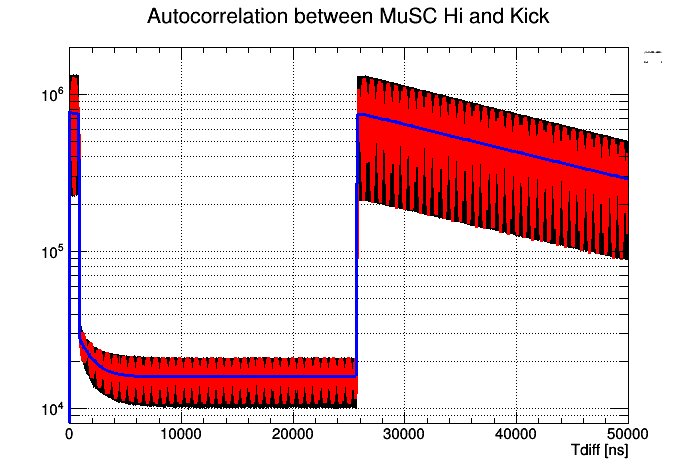
\includegraphics[width=\textwidth]{beam/figures/MuSC_Kick_Corr.png}
  \caption{Fit to entrance vs kick correlation plot.  The data is shown in black, the fit is in red, and blue shows the fit with the oscillations disabled.}
  \label{fig:musc_fit}
\end{figure}

\begin{table}[h]
  \begin{center}
    \caption{Muon background fit parameters}
    \label{tab:mu_params}
    \begin{tabular}{ | l | r | r | }
      \hline
      Parameter   & Value       & Error       \\
      \hline
      A           & 741008      & 13 \\
      B           & 532157      & 12 \\
      C           & 15925       & 1 \\
      D           & 5167.8      & 1.3 \\
      $\sigma$    & 28.8216     & 8.95785e-03 \\
      $\omega_b$  & 0.318511    & 1.84633e-09 \\
      $\phi_b$    & 1.58975     & 0.00007     \\
      $\phi_k$    & 1.21904     & 0.00025     \\
      $\lambda_b$ & 4.15123e-05 & 1.52711e-09 \\
      $t_{k}$     & 25723.9     & 8.10876e-03 \\
      $t_{\mu}$   & 822.676     & 7.22884e-03 \\
      \hline
    \end{tabular}
  \end{center}
\end{table}

\section{Neutron Background}

Next, we will consider beam neutrons.
These neutrons are produced by muons which stop upstream of the detector anywhere in the beam pipe or collimators.
The muons then undergo nuclear capture and emit neutrons with a fast exponential time distribution.
Convolving this with the kicker time distribution produces a smeared version:
\begin{equation}
P_{b,n}(t) = \begin{cases} \frac{\lambda_w}{\lambda_b + \lambda_w} e^{\lambda_b t}                            & -t_k+t_{\mu}<t<0 \\
1 - \frac{\lambda_b}{\lambda_b + \lambda_w} e^{-\lambda_w t}                       & 0<t<t_{\mu} \\
(e^{\lambda_w t_{\mu}} - \frac{\lambda_b}{\lambda_b + \lambda_w}) e^{-\lambda_w t} & t_{\mu}<t<t_k-t_{\mu} \end{cases}
\label{eq:kicker_neutron}
\end{equation}

There is a time offset relative to the muon signal, which depends on both the emission location and on the energy of the neutron and could be complicated to model.
There could also be several sources with different capture rates and distances to the detectors.
However, the neutrons are emitted from stopped muons and have no preferred direction, so the contribution from upstream sources falls off with the square of the distance.
This means the shape of the neutron background is dominated by stops in the lead collimator on the entrance detector stack.
The proximity of the source to the detectors means the neutron time of flight is not very significant, and they closely match the delay of the muons.
The next most prominent source of neutrons should be the collimator in the bending magnet, but this has not been observed due to low statistics.

Finally, the random delays involved in neutron emission seem to be effective at averaging out the effects of the accelerator RF oscillations as far as we can determine with available statistics.
Therefore, I omit the oscillating term in the background model for the neutrons.  
The neutron background is then simply given by:
\begin{equation}
R_n(t) = A P_{b,n}(t+\Delta t_n) + B (1-P_{b,n}(t+\Delta t_n)).
\label{eq:neutron}
\end{equation}
The parameters $\lambda_w$, $\Delta t_n$, A, and B must be fit to match the neutron background, see chapter \ref{ch:neutrons} for details.

\section{Electron Background}

The beam electron background is extremely important since it directly enters the lifetime histograms.  
The signal due to electrons produced upstream of the kicker may be modeled as the combination of kicked and un-kicked beams in the same way as the muon backgrounds.
In this case, the only differences from the muon background model are consequences of the time of flight.
The 40 $MeV/c$ muons in the beam only travel at about one third the speed of light, but the electrons travel at nearly the speed of light.
This speed difference means electrons from the kicker arrive at the detectors sooner than muons, shifting the kicker time dependence earlier.
It also results in a phase shift in the electron background RF oscillations depending on where in the beam the electrons were emitted.

However, a complication arises when we consider muons which pass the kicker before firing.
Because of this speed difference between the muons and electrons, the time dependence of these electrons will be offset depending on the source location.
For muons that decay in flight, the expected signal is obtained by starting with an exponential decay and then transforming from the decay time to the observed time:
\begin{align}
P_e(t) & = \gamma \lambda_{\mu} e^{\gamma \lambda_{\mu} t} * [A + B sin(\omega_b t + \phi)]\\
t_{obs} & = t + (d-x(t))/c = (d/c+(1-\beta)t) \\
P_e(t_{obs}) & = \gamma \lambda_{\mu} e^{\gamma \lambda_{\mu} (t_{obs}-d/c)/(1-\beta)} * [A + B sin(\omega_b (t_{obs}-d/c)/(1-\beta) + \phi)]
\end{align}

We must also consider background electrons produced by muon decays in the collimators or beam pipe.  
This component of the electron background should have a time distribution much like the neutron background, which was also produced by upstream wall stops.
However, since electrons will move differently than neutrons under the influence of the beam magnets we expect such signals to have different strengths.

Another complication is that transient effects when the kicker activates are now a real possibility.
Because the electron detectors form a cylinder surrounding the beam, when the beam is deflected it could briefly produce an increased signal as it sweeps across the detectors.
With the muon clock we have observed some evidence of a bump in the background observed during the kicker step, although this may be explained by the combination of multiple background components.
For now I will assume the same error function transition as for the muons, but this should be studied further.
%todo - study it

An interesting feature of the beam electron background is that for most datasets the kicked background rate is observed to be higher than the un-kicked rate.
Two possible explanations for this effect are apparent.
One scenario is that the kicked configuration happens to divert the beam electrons directly into the electron detectors, while they would pass through the center without being detected when the kicker is off.
Alternatively, when the beam is diverted into the upstream collimator it may produce a large number of additional background electrons.
These cases may be distinguishable by studying the amplitude of the beam RF oscillations as well as any vertical deflection produced by the kicker.
%todo - add anything important from Peter and Rachel elogs

\section{Gamma Background}

The last background type we will consider is the gamma ray background.
Gamma rays are most likely bremsstrahlung radiation, probably emitted from the bending magnet that sends the beam into the detectors.
Bremsstrahlung radiation depends on the velocity and acceleration of the particles, so the signal should be dominated by electrons rather than muons.
The gamma ray background therefore shares many features of the electron background.
However, for our purposes it is not necessary to model the gamma background in nearly as much detail as the electrons, so we use a single kicker step:
%todo - compare gamma and electron backgrounds.
\begin{equation}
R_{\gamma}(t) = [A + B sin(\omega_b t + \phi)] * P_{b,\mu}(+\Delta t_{\gamma}) + [C + D sin(\omega_b t + \phi)] * P_{b,\mu}(+\Delta t_{\gamma})
\end{equation}

\section{Combined Backgrounds}

Finally, it is possible to have multiple sources of background present at once.
For example, the neutron detectors are sensitive to both neutrons and gamma rays.
Because the kicker reduces the entrance rates of muons and neutrons but increases them for electrons and gammas, the sum of these signals can have an interesting result.
For the most part, the opposite signals simply cancel out, but the differences in time of flight mean that the gammas switch to the kicked state before the neutrons.
Thus, we have a brief period where the gamma rate has increased but the neutron rate has not dropped yet, producing a spike in the background as shown in figure \ref{fig:finger}.

\begin{figure}[h]
  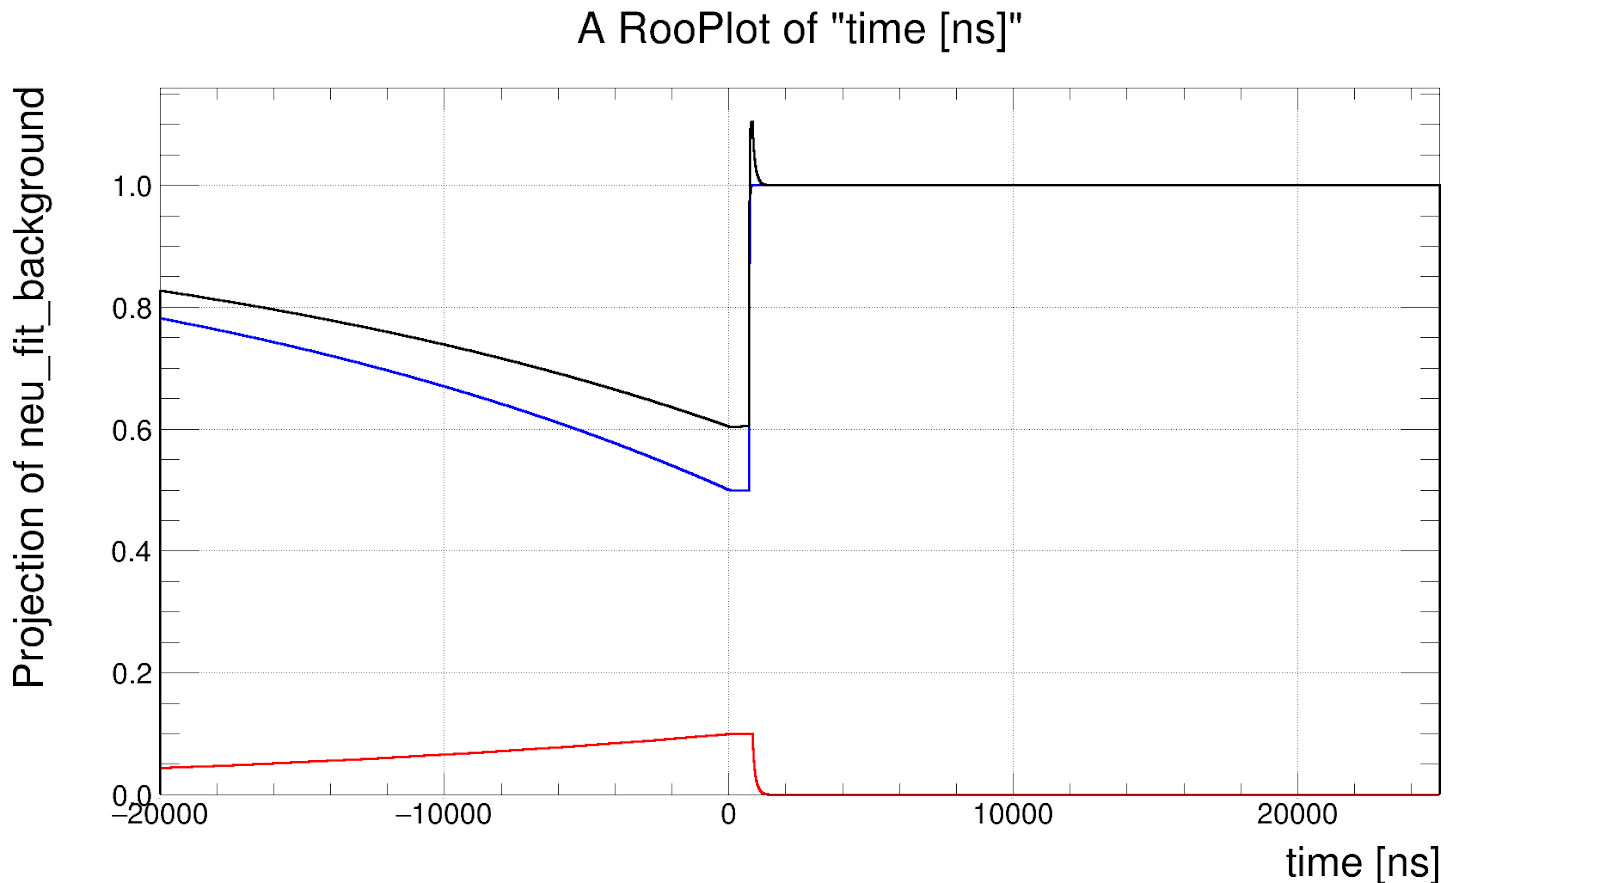
\includegraphics[width=\textwidth]{beam/figures/Finger_Model.png}
  \caption{Background spike produced by the sum (black) of neutron (red) and gamma (blue) signals. }
  \label{fig:finger}
\end{figure}

An analogous effect can also occur with the muon and electron signal, for any detectors sensitive to both.
It is also possible to see the effect with electrons alone, if we have a significant number of background electrons coming from nearby stops in the area producing a downward kick after the main upward kick.
This signal can be distinguished from the possible transient spike mentioned earlier because this peak is much longer.  
A background spike produced by the kicker can only last a few $ns$ as the kicker charges, whereas this combined background peak can be more than 100 $ns$.